\documentclass[10pt]{article}
\usepackage[T1]{fontenc}
\usepackage[utf8]{inputenc}
%\DeclareUnicodeCharacter{00A0}{ }
%\usepackage[adobe-utopia]{mathdesign}

\usepackage{amsmath}
\usepackage[francais]{babel}
\usepackage[dvips]{graphicx}
%\usepackage{here}
\usepackage{framed}
\usepackage[normalem]{ulem}
\usepackage{fancyhdr}
\usepackage{titlesec}
\usepackage{vmargin}

\usepackage{amsmath}
\usepackage{ifthen}
\usepackage{multirow}
\usepackage{multicol} % Portions de texte en colonnes

%\usepackage{xltxtra} % Logo XeLaTeX
%\usepackage{pst-solides3d}
\usepackage{color}
%\usepackage{colortbl}
\usepackage{titletoc} % Pour la mise en forme de la table des matières

%\usepackage[crop=off]{auto-pst-pdf}
%\usepackage{bclogo}


%\usepackage{longtable}
%\usepackage{flafter}%floatants après la référence
%\usepackage{pst-solides3d}
%\usepackage{pstricks}
%\usepackage{minitoc}
%\setcounter{minitocdepth}{4}
%\usepackage{draftcopy}% "Brouillon"
%\usepackage{floatflt}
%\usepackage{psfrag}
%\usepackage{listings} % Permet d'insérer du code de programmation
%\usepackage{lmodern}
%\usepackage[adobe-utopia,uppercase=upright,greeklowercase=upright]{mathdesign}
%\usepackage{minionpro}
%\usepackage{pifont}
%\usepackage{amssymb}
%\usepackage[francais]{varioref}

\setmarginsrb{1.5cm}{1cm}{1cm}{1.5cm}{1cm}{1cm}{1cm}{1cm}

\definecolor{gris25}{gray}{0.75}
\definecolor{bleu}{RGB}{18,33,98}
\definecolor{bleuf}{RGB}{42,94,171}
\definecolor{bleuc}{RGB}{231,239,247}
\definecolor{rougef}{RGB}{185,18,27}
\definecolor{rougec}{RGB}{255,230,231}
\definecolor{vertf}{RGB}{103,126,82}
\definecolor{vertc}{RGB}{220,255,191}
\definecolor{violetf}{RGB}{112,48,160}
\definecolor{violetc}{RGB}{230,224,236}
\definecolor{jaunec}{RGB}{220,255,191}
%\usepackage{algorithm}
%\usepackage{algorithmic}
\usepackage[french]{algorithm2e}

\SetKwBlock{Fonction}{Début Fonction}{Fin Fonction}
\SetKwComment{Comment}{start}{end}
% Python sources

\usepackage{listings}
\lstloadlanguages{R}   % pour regler les pb d accent utf8 dans les codes
\lstset{language=R} % pour regler les pb d accent utf8 dans les codes

\usepackage{textcomp}
\usepackage{setspace}
%\usepackage{palatino}

%\usepackage{color}
\definecolor{Bleu}{rgb}{0.1,0.1,1.0}
\definecolor{Noir}{rgb}{0,0,0}
\definecolor{Grau}{rgb}{0.5,0.5,0.5}
\definecolor{DunkelGrau}{rgb}{0.15,0.15,0.15}
\definecolor{Hellbraun}{rgb}{0.5,0.25,0.0}
\definecolor{Magenta}{rgb}{1.0,0.0,1.0}
\definecolor{Gris}{gray}{0.5}
\definecolor{Vert}{rgb}{0,0.5,0}
\definecolor{SourceHintergrund}{rgb}{1,1.0,0.95}


%
\renewcommand{\lstlistlistingname}{Listings}
\renewcommand{\lstlistingname}{Listing}

\lstnewenvironment{python}[1][]{
\lstset{
%escapeinside={\%*}{*)},
%inputencoding=utf8,   % pour regler les pb d accent utf8 dans les codes
%extendedchars=true,   % pour regler les pb d accent utf8 dans les codes
language=python,
basicstyle=\sffamily\footnotesize, 	
stringstyle=\color{red}, 
showstringspaces=false, 
alsoletter={1234567890},
otherkeywords={\ , \}, \{},
keywordstyle=\color{blue},
emph={access,and,break,class,continue,def,del,elif ,else,
except,exec,finally,for,from,global,if,import,in,i s,
lambda,not,or,pass,print,raise,return,try,while},
emphstyle=\color{black}\bfseries,
emph={[2]True, False, None, self},
emphstyle=[2]\color{olive},
emph={[3]from, import, as},
emphstyle=[3]\color{blue},
upquote=true,
columns=flexible, % pour empecher d'avoir un espacement mono
morecomment=[s]{"""}{"""},
commentstyle=\color{Hellbraun}\slshape, 
%emph={[4]1, 2, 3, 4, 5, 6, 7, 8, 9, 0},
emphstyle=[4]\color{blue},
literate=*{:}{{\textcolor{blue}:}}{1}
{=}{{\textcolor{blue}=}}{1}
{-}{{\textcolor{blue}-}}{1}
{+}{{\textcolor{blue}+}}{1}
{*}{{\textcolor{blue}*}}{1}
{!}{{\textcolor{blue}!}}{1}
{(}{{\textcolor{blue}(}}{1}
{)}{{\textcolor{blue})}}{1}
{[}{{\textcolor{blue}[}}{1}
{]}{{\textcolor{blue}]}}{1}
{<}{{\textcolor{blue}<}}{1}
{>}{{\textcolor{blue}>}}{1}
{COMPLETER}{{\textcolor{red}COMPLETER}}{1},
literate=%
            {é}{{\'{e}}}1
            {è}{{\`{e}}}1
            {ê}{{\^{e}}}1
            {ë}{{\¨{e}}}1
            {û}{{\^{u}}}1
            {ù}{{\`{u}}}1
            {â}{{\^{a}}}1
            {à}{{\`{a}}}1
            {î}{{\^{i}}}1
            {ç}{{\c{c}}}1
            {Ç}{{\c{C}}}1
            {É}{{\'{E}}}1
            {Ê}{{\^{E}}}1
            {À}{{\`{A}}}1
            {Â}{{\^{A}}}1
            {Î}{{\^{I}}}1, % pour regler les pb d accent utf8 dans les codes
%framexleftmargin=1mm, framextopmargin=1mm, frame=shadowbox, rulesepcolor=\color{blue},#1
%backgroundcolor=\color{SourceHintergrund}, 
%framexleftmargin=1mm, framexrightmargin=1mm, framextopmargin=1mm, frame=single, framerule=1pt, rulecolor=\color{black},#1
}}{}



\lstnewenvironment{scilab}[1][]{
\lstset{
language=scilab,
basicstyle=\sffamily\footnotesize, 	
stringstyle=\color{red}, 
showstringspaces=false, 
alsoletter={1234567890},
otherkeywords={\ , \}, \{},
keywordstyle=\color{blue},
emph={access,and,break,class,continue,def,del,elif ,else,
except,exec,finally,for,from,global,if,import,in,i s,
lambda,not,or,pass,print,raise,return,try,while,Debut},
emphstyle=\color{black}\bfseries,
emph={[2]True, False, None, self},
emphstyle=[2]\color{olive},
emph={[3]from, import, as},
emphstyle=[3]\color{blue},
upquote=true,
columns=flexible, % pour empecher d'avoir un espacement mono
morecomment=[s]{"""}{"""},
commentstyle=\color{Hellbraun}\slshape, 
%emph={[4]1, 2, 3, 4, 5, 6, 7, 8, 9, 0},
emphstyle=[4]\color{blue},
literate=*{:}{{\textcolor{blue}:}}{1}
{=}{{\textcolor{blue}=}}{1}
{-}{{\textcolor{blue}-}}{1}
{+}{{\textcolor{blue}+}}{1}
{*}{{\textcolor{blue}*}}{1}
{!}{{\textcolor{blue}!}}{1}
{(}{{\textcolor{blue}(}}{1}
{)}{{\textcolor{blue})}}{1}
{[}{{\textcolor{blue}[}}{1}
{]}{{\textcolor{blue}]}}{1}
{<}{{\textcolor{blue}<}}{1}
{>}{{\textcolor{blue}>}}{1},
%framexleftmargin=1mm, framextopmargin=1mm, frame=shadowbox, rulesepcolor=\color{blue},#1
%backgroundcolor=\color{SourceHintergrund}, 
%framexleftmargin=1mm, framexrightmargin=1mm, framextopmargin=1mm, frame=single, framerule=1pt, rulecolor=\color{black},#1
}}{}


\lstdefinestyle{stylepython}{%
escapeinside={\%*}{*)},
inputencoding=utf8,   % pour regler les pb d accent utf8 dans les codes
extendedchars=true,   % pour regler les pb d accent utf8 dans les codes
language=python,
basicstyle=\sffamily\footnotesize, 	
stringstyle=\color{red}, 
showstringspaces=false, 
alsoletter={1234567890},
otherkeywords={\ , \}, \{},
keywordstyle=\color{blue},
emph={access,and,break,class,continue,def,del,elif ,else,
except,exec,finally,for,from,global,if,import,in,i s,
lambda,not,or,pass,print,raise,return,try,while},
emphstyle=\color{black}\bfseries,
emph={[2]True, False, None, self},
emphstyle=[2]\color{green},
emph={[3]from, import, as},
emphstyle=[3]\color{blue},
upquote=true,
columns=flexible, % pour empecher d'avoir un espacement mono
morecomment=[s]{"""}{"""},
commentstyle=\color{Hellbraun}\slshape, 
%emph={[4]1, 2, 3, 4, 5, 6, 7, 8, 9, 0},
emphstyle=[4]\color{blue},
literate=*{:}{{\textcolor{blue}:}}{1}
{=}{{\textcolor{blue}=}}{1}
{-}{{\textcolor{blue}-}}{1}
{+}{{\textcolor{blue}+}}{1}
{*}{{\textcolor{blue}*}}{1}
{!}{{\textcolor{blue}!}}{1}
{(}{{\textcolor{blue}(}}{1}
{)}{{\textcolor{blue})}}{1}
{[}{{\textcolor{blue}[}}{1}
{]}{{\textcolor{blue}]}}{1}
{<}{{\textcolor{blue}<}}{1}
{>}{{\textcolor{blue}>}}{1}
{COMPLETER}{{\textcolor{red}COMPLETER}}{1},
literate=%
            {é}{{\'{e}}}1
            {è}{{\`{e}}}1
            {ê}{{\^{e}}}1
            {ë}{{\¨{e}}}1
            {û}{{\^{u}}}1
            {ù}{{\`{u}}}1
            {â}{{\^{a}}}1
            {à}{{\`{a}}}1
            {î}{{\^{i}}}1
            {ç}{{\c{c}}}1
            {Ç}{{\c{C}}}1
            {É}{{\'{E}}}1
            {Ê}{{\^{E}}}1
            {À}{{\`{A}}}1
            {Â}{{\^{A}}}1
            {Î}{{\^{I}}}1,
%numbers=left,                    % where to put the line-numbers; possible values are (none, left, right)
%numbersep=5pt,                   % how far the line-numbers are from the code
%numberstyle=\tiny\color{mygray}, % the style that is used for the line-numbers
}

%
%\renewcommand{\algorithmicrequire} {\textbf{\textsc{Entrées:}}}
%\renewcommand{\algorithmicensure}  {\textbf{\textsc{Sorties:}}}
%\renewcommand{\algorithmicwhile}   {\textbf{tantque}}
%\renewcommand{\algorithmicdo}      {\textbf{faire}}
%\renewcommand{\algorithmicendwhile}{\textbf{fin tantque}}
%\renewcommand{\algorithmicend}     {\textbf{fin}}
%\renewcommand{\algorithmicif}      {\textbf{si}}
%\renewcommand{\algorithmicendif}   {\textbf{finsi}}
%\renewcommand{\algorithmicelse}    {\textbf{sinon}}
%\renewcommand{\algorithmicthen}    {\textbf{alors}}
%\renewcommand{\algorithmicfor}     {\textbf{pour}}
%\renewcommand{\algorithmicforall}  {\textbf{pour tout}}
%\renewcommand{\algorithmicdo}      {\textbf{faire}}
%\renewcommand{\algorithmicendfor}  {\textbf{fin pour}}
%\renewcommand{\algorithmicloop}    {\textbf{boucler}}
%\renewcommand{\algorithmicendloop} {\textbf{fin boucle}}
%\renewcommand{\algorithmicrepeat}  {\textbf{répéter}}
%\renewcommand{\algorithmicuntil}   {\textbf{jusqu'à}}

\lstnewenvironment{termi}[1][]{
\lstset{
language=scilab,
basicstyle=\sffamily\footnotesize, 	
stringstyle=\color{red}, 
showstringspaces=false, 
alsoletter={1234567890},
otherkeywords={\ , \}, \{},
keywordstyle=\color{blue},
emph={access,and,break,class,continue,def,del,elif ,else,
except,exec,finally,for,from,global,if,import,in,i s,
lambda,not,or,pass,print,raise,return,try,while,Debut},
emphstyle=\color{black}\bfseries,
emph={[2]True, False, None, self},
emphstyle=[2]\color{green},
emph={[3]from, import, as},
emphstyle=[3]\color{blue},
upquote=true,
columns=flexible, % pour empecher d'avoir un espacement mono
morecomment=[s]{"""}{"""},
commentstyle=\color{Hellbraun}\slshape, 
%emph={[4]1, 2, 3, 4, 5, 6, 7, 8, 9, 0},
emphstyle=[4]\color{blue},
literate=*{:}{{\textcolor{blue}:}}{1}
{=}{{\textcolor{blue}=}}{1}
{-}{{\textcolor{blue}-}}{1}
{+}{{\textcolor{blue}+}}{1}
{*}{{\textcolor{blue}*}}{1}
{!}{{\textcolor{blue}!}}{1}
{(}{{\textcolor{blue}(}}{1}
{)}{{\textcolor{blue})}}{1}
{[}{{\textcolor{blue}[}}{1}
{]}{{\textcolor{blue}]}}{1}
{<}{{\textcolor{blue}<}}{1}
{>}{{\textcolor{blue}>}}{1},
%framexleftmargin=1mm, framextopmargin=1mm, frame=shadowbox, rulesepcolor=\color{blue},#1
%backgroundcolor=\color{SourceHintergrund}, 
%framexleftmargin=1mm, framexrightmargin=1mm, framextopmargin=1mm, frame=single, framerule=1pt, rulecolor=\color{black},#1
}}{}


%
%\renewcommand{\algorithmicrequire} {\textbf{\textsc{Entrées:}}}
%\renewcommand{\algorithmicensure}  {\textbf{\textsc{Sorties:}}}
%\renewcommand{\algorithmicwhile}   {\textbf{tantque}}
%\renewcommand{\algorithmicdo}      {\textbf{faire}}
%\renewcommand{\algorithmicendwhile}{\textbf{fin tantque}}
%\renewcommand{\algorithmicend}     {\textbf{fin}}
%\renewcommand{\algorithmicif}      {\textbf{si}}
%\renewcommand{\algorithmicendif}   {\textbf{finsi}}
%\renewcommand{\algorithmicelse}    {\textbf{sinon}}
%\renewcommand{\algorithmicthen}    {\textbf{alors}}
%\renewcommand{\algorithmicfor}     {\textbf{pour}}
%\renewcommand{\algorithmicforall}  {\textbf{pour tout}}
%\renewcommand{\algorithmicdo}      {\textbf{faire}}
%\renewcommand{\algorithmicendfor}  {\textbf{fin pour}}
%\renewcommand{\algorithmicloop}    {\textbf{boucler}}
%\renewcommand{\algorithmicendloop} {\textbf{fin boucle}}
%\renewcommand{\algorithmicrepeat}  {\textbf{répéter}}
%\renewcommand{\algorithmicuntil}   {\textbf{jusqu'à}}
%%%%%%%%%%%%
% Définition des vecteurs 
%%%%%%%%%%%%
 \newcommand{\vect}[1]{\overrightarrow{#1}}

%%%%%%%%%%%%
% Définition des torseurs 
%%%%%%%%%%%%

 \newcommand{\torseur}[1]{%
\left\{{#1}\right\}
}

\newcommand{\torseurcin}[3]{%
\left\{\mathcal{#1} \left(#2/#3 \right) \right\}
}

\newcommand{\torseurstat}[3]{%
\left\{\mathcal{#1} \left(#2\rightarrow #3 \right) \right\}
}

 \newcommand{\torseurc}[8]{%
%\left\{#1 \right\}=
\left\{
{#1}
\right\}
 = 
\left\{%
\begin{array}{cc}%
{#2} & {#5}\\%
{#3} & {#6}\\%
{#4} & {#7}\\%
\end{array}%
\right\}_{#8}%
}

 \newcommand{\torseurcol}[7]{
\left\{%
\begin{array}{cc}%
{#1} & {#4}\\%
{#2} & {#5}\\%
{#3} & {#6}\\%
\end{array}%
\right\}_{#7}%
}

 \newcommand{\torseurl}[3]{%
%\left\{\mathcal{#1}\right\}_{#2}=%
\left\{%
\begin{array}{l}%
{#1} \\%
{#2} %
\end{array}%
\right\}_{#3}%
}

 \newcommand{\vectv}[3]{%
\vect{V\left( {#1} \in {#2}/{#3}\right)}
}


\newcommand{\vectf}[2]{%
\vect{R\left( {#1} \rightarrow {#2}\right)}
}

\newcommand{\vectm}[3]{%
\vect{\mathcal{M}\left( {#1}, {#2} \rightarrow {#3}\right)}
}


 \newcommand{\vectg}[3]{%
\vect{\Gamma \left( {#1} \in {#2}/{#3}\right)}
}

 \newcommand{\vecto}[2]{%
\vect{\Omega\left( {#1}/{#2}\right)}
}
% }$$\left\{\mathcal{#1} \right\}_{#2} =%
% \left\{%
% \begin{array}{c}%
%  #3 \\%
%  #4 %
% \end{array}%
% \right\}_{#5}}
\setcounter{tocdepth}{2}
% \mtcselectlanguage{french} 


%  ------------------------------------------
% | Modification du formatage des sections : | 
%  ------------------------------------------

% Grands titres :
% ---------------

\newcommand{\titre}[1]{%
\begin{center}
      \bigskip
      \rule{\textwidth}{1pt}
      \par\vspace{0.1cm}
      
      \textbf{\large #1}
      \par\rule{\textwidth}{1pt}
    \end{center}
    \bigskip
  }

% Supprime le numéro du chapitre dans la numérotation des sections:
% -----------------------------------------------------------------
\makeatletter
\renewcommand{\thesection}{\@arabic\c@section}
\makeatother


% \titleformat{\chapter}[display]
% {\normalfont\Large\filcenter}
% {}
% {1pc}
% {\titlerule[1pt]
%   \vspace{1pc}%
%   \Huge}[\vspace{1ex}%
% \titlerule]


%%%% Chapitres Comme PY Pechard %%%%%%%%%
% numéro du chapitre
\DeclareFixedFont{\chapnumfont}{OT1}{phv}{b}{n}{80pt}
% pour le mot « Chapitre »
\DeclareFixedFont{\chapchapfont}{OT1}{phv}{m}{it}{40pt}
% pour le titre
\DeclareFixedFont{\chaptitfont}{T1}{phv}{b}{n}{25pt}

\definecolor{gris}{gray}{0.75}
\titleformat{\chapter}[display]%
	{\sffamily}%
	{\filleft\chapchapfont\color{gris}\chaptertitlename\
	\\
	\vspace{12pt}
	\chapnumfont\thechapter}%
	{16pt}%
	{\filleft\chaptitfont}%
	[\vspace{6pt}\titlerule\titlerule\titlerule]

%%%%  Fin Chapitres Comme PY Pechard %%%%%%%%%


% Section, subsection, subsubsection sans serifs :
% % ----------------------------------------------

% \makeatletter
% \renewcommand{\section}{\@startsection{section}{0}{0mm}%
% {\baselineskip}{.3\baselineskip}%
% {\normalfont\sffamily\Large\textbf}}%
% \makeatother

\makeatletter
\renewcommand{\@seccntformat}[1]{{\textcolor{bleu}{\csname
the#1\endcsname}\hspace{0.5em}}}
\makeatother

\makeatletter
\renewcommand{\section}{\@startsection{section}{1}{\z@}%
                       {-4ex \@plus -1ex \@minus -.4ex}%
                       {1ex \@plus.2ex }%
                       {\normalfont\Large\sffamily\bfseries}}%
\makeatother
 
\makeatletter
\renewcommand{\subsection}{\@startsection {subsection}{2}{\z@}
                          {-3ex \@plus -0.1ex \@minus -.4ex}%
                          {0.5ex \@plus.2ex }%
                          {\normalfont\large\sffamily\bfseries}}
\makeatother
 
\makeatletter
\renewcommand{\subsubsection}{\@startsection {subsubsection}{3}{\z@}
                          {-2ex \@plus -0.1ex \@minus -.2ex}%
                          {0.2ex \@plus.2ex }%
                          {\normalfont\large\sffamily\bfseries}}
\makeatother
 
\makeatletter             
\renewcommand{\paragraph}{\@startsection{paragraph}{4}{\z@}%
                                    {-2ex \@plus-.2ex \@minus .2ex}%
                                    {0.1ex}%               
{\normalfont\sffamily\bfseries}}
\makeatother
 
 
\makeatletter             
\renewcommand{\subparagraph}{\@startsection{subparagraph}{5}{\z@}%
                                    {-2ex \@plus-.2ex \@minus .2ex}%
                                    {0ex}%               
{\normalfont\bfseries Question }}
\makeatother
\renewcommand{\thesubparagraph}{\arabic{subparagraph}} 
\makeatletter

\setcounter{secnumdepth}{5}





% Formatage de la table des matières 
% Paquets nécessaires : titletoc ?

% Chapitre spéciaux écrits dans un nombre cerclé dans la table des matières.
\titlecontents{chapter}[+3pc]
  {\addvspace{10pt}\sffamily\bfseries}
{\contentslabel[{\pscirclebox[fillstyle=solid,fillcolor=gray!25,
linecolor=gray!25,framesep=4pt]{\textcolor{white}{\thecontentslabel}}}]{2.5pc}}
  {}
  {\dotfill \normalfont\thecontentspage\ }

\titlecontents{section}[3pc]
  {\addvspace{2pt}\sffamily}
  {\contentslabel[\thecontentslabel]{1.8pc}}
  {}
  {\dotfill \normalfont\thecontentspage\ }

\titlecontents{subsection}[5pc]
  {\addvspace{2pt}\sffamily}
  {\contentslabel[\thecontentslabel]{1.8pc}}
  {}
  {\dotfill \normalfont\thecontentspage\ }

\titlecontents{subsubsection}[8pc]
  {\addvspace{2pt}\sffamily}
  {\contentslabel[\thecontentslabel]{3pc}}
  {}
  {\dotfill \normalfont\thecontentspage\ }
%{\;\titlerule\;\normalfont\thecontentspage\ }

\titlecontents{paragraph}[9pc]
  {\addvspace{2pt}\sffamily}
  {\contentslabel[\thecontentslabel]{3.5pc}}
  {}
  {\dotfill \normalfont\thecontentspage\ }

%pour avoir l indentation dans minipage
\newdimen\oldparindent\oldparindent=\parindent

\makeatletter
\def\@iiiminipage#1#2[#3]#4{%
  \noindent
  \leavevmode
  \@pboxswfalse
  \setlength\@tempdima{#4}%
  \def\@mpargs{{#1}{#2}[#3]{#4}}%
  \setbox\@tempboxa\vbox\bgroup
    \color@begingroup
      \hsize\@tempdima
      \textwidth\hsize \columnwidth\hsize
      \@parboxrestore
      \parindent=\oldparindent
      \def\@mpfn{mpfootnote}\def\thempfn{\thempfootnote}\c@mpfootnote\z@
      \let\@footnotetext\@mpfootnotetext
      \let\@listdepth\@mplistdepth \@mplistdepth\z@
      \@minipagerestore
      \@setminipage}
\makeatother

% Paquets requis : 

\definecolor{gris25}{gray}{0.75}
\definecolor{bleu}{RGB}{18,33,98}
\definecolor{bleuf}{RGB}{42,94,171}
\definecolor{bleuc}{RGB}{231,239,247}
\definecolor{rougef}{RGB}{185,18,27}
\definecolor{rougec}{RGB}{255,230,231}
\definecolor{vertf}{RGB}{103,126,82}
\definecolor{vertc}{RGB}{220,255,191}
\definecolor{violetf}{RGB}{112,48,160}
\definecolor{violetc}{RGB}{230,224,236}
\definecolor{jaunec}{RGB}{220,255,191}



\newenvironment{corrige}[1][\hsize]%
{%
    \def\FrameCommand%
    {%
\rotatebox{90}{\textit{\textsf{Corrigé}}} 
        {\color{violetf}\vrule width 3pt}%
        \hspace{0pt}%must no space.
        \fboxsep=\FrameSep\colorbox{violetc}%
    }%
    \MakeFramed{\hsize #1 \advance\hsize-\width\FrameRestore}%
}%
{\endMakeFramed}%

\newenvironment{sci}[1][\hsize]%
{%
    \def\FrameCommand%
    {%
%\rotatebox{90}{\textit{\textsf{Scilab}}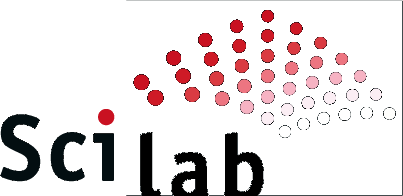
\includegraphics[height=.8cm]{png/logo_scilab}} 
\rotatebox{90}{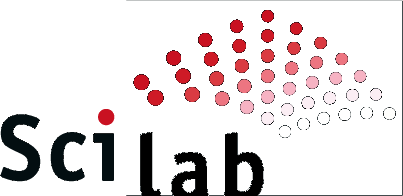
\includegraphics[height=.6cm]{png/logo_scilab}} 
        {\color{violetf}\vrule width 3pt}%
        \hspace{0pt}%must no space.
        \fboxsep=\FrameSep\colorbox{violetc}%
    }%
    \MakeFramed{\hsize #1 \advance\hsize-\width\FrameRestore}%
}%
{\endMakeFramed}%

\newenvironment{pseudo}[1][\hsize]%
{%
    \def\FrameCommand%
    {%
\rotatebox{90}{\textit{\textsf{Pseudo Code}}} 
        {\color{violetf}\vrule width 3pt}%
        \hspace{0pt}%must no space.
        \fboxsep=\FrameSep\colorbox{violetc}%
    }%
    \MakeFramed{\hsize #1 \advance\hsize-\width\FrameRestore}%
}%
{\endMakeFramed}%

\newenvironment{py}[1][\hsize]%
{%
    \def\FrameCommand%
    {%
%\rotatebox{90}{\textit{\textsf{Python}}} 
\rotatebox{90}{
\includegraphics[height=.6cm]{png/logo_python}} 
        {\color{violetf}\vrule width 3pt}%
        \hspace{0pt}%must no space.
        \fboxsep=\FrameSep\colorbox{violetc}%
    }%
    \MakeFramed{\hsize #1 \advance\hsize-\width\FrameRestore}%
}%
{\endMakeFramed}%


\newenvironment{term}[1][\hsize]%
{%
    \def\FrameCommand%
    {%
\rotatebox{90}{\textit{\textsf{Terminal}}} 
        {\color{violetf}\vrule width 3pt}%
        \hspace{0pt}%must no space.
        \fboxsep=\FrameSep\colorbox{violetc}%
    }%
    \MakeFramed{\hsize #1 \advance\hsize-\width\FrameRestore}%
}%
{\endMakeFramed}%



\newenvironment{comp}[1][\hsize]%
{%
    \def\FrameCommand
    {%
\rotatebox{90}{\textit{\textsf{Compétences}}} 
        {\color{bleuf}\vrule width 3pt}%
        \hspace{0pt}%must no space.
        \fboxsep=\FrameSep\colorbox{bleuc}%
    }%
    \MakeFramed{\hsize#1\advance\hsize-\width\FrameRestore}%
}%
{\endMakeFramed}%

\newenvironment{rem}[1][\hsize]%
{%
    \def\FrameCommand
    {%
\rotatebox{90}{\textit{\textsf{Remarque}}} 
        {\color{bleuf}\vrule width 3pt}%
        \hspace{0pt}%must no space.
        \fboxsep=\FrameSep\colorbox{bleuc}%
    }%
    \MakeFramed{\hsize#1\advance\hsize-\width\FrameRestore}%
}%
{\endMakeFramed}%


\newenvironment{savoir}[1][\hsize]%
{%
    \def\FrameCommand
    {%
\rotatebox{90}{\textit{\textsf{Savoir}}} 
        {\color{bleuf}\vrule width 3pt}%
        \hspace{0pt}%must no space.
        \fboxsep=\FrameSep\colorbox{bleuc}%
    }%
    \MakeFramed{\hsize#1\advance\hsize-\width\FrameRestore}%
}%
{\endMakeFramed}%

\newenvironment{Objectif}[1][\hsize]%
{%
    \def\FrameCommand
    {%
\rotatebox{90}{\textit{\textsf{Objectif}}} 
        {\color{bleuf}\vrule width 3pt}%
        \hspace{0pt}%must no space.
        \fboxsep=\FrameSep\colorbox{bleuc}%
    }%
    \MakeFramed{\hsize#1\advance\hsize-\width\FrameRestore}%
}%
{\endMakeFramed}%

\newenvironment{prob}[1][\hsize]%
{%
    \def\FrameCommand%
    {%
\rotatebox{90}{\textit{\textsf{ Problématique}}} 
        {\color{rougef}\vrule width 3pt}%
        \hspace{0pt}%must no space.
        \fboxsep=\FrameSep\colorbox{rougec}%
    }%
    \MakeFramed{\hsize#1\advance\hsize-\width\FrameRestore}%
}%
{\endMakeFramed}%

\newenvironment{obj}[1][\hsize]%
{%
    \def\FrameCommand%
    {%
\rotatebox{90}{\textit{\textsf{Objectifs}}} 
        {\color{rougef}\vrule width 3pt}%
        \hspace{0pt}%must no space.
        \fboxsep=\FrameSep\colorbox{rougec}%
    }%
    \MakeFramed{\hsize#1\advance\hsize-\width\FrameRestore}%
}%
{\endMakeFramed}%

\newenvironment{defi}[1][\hsize]%
{%
    \def\FrameCommand%
    {%
\rotatebox{90}{\textit{\textsf{Définition\\}}} 
        {\color{bleuf}\vrule width 3pt}%
        \hspace{0pt}%must no space.
        \fboxsep=\FrameSep\colorbox{bleuc}%
    }%
    \MakeFramed{\hsize#1\advance\hsize-\width\FrameRestore}%
}%
{\endMakeFramed}%


\newenvironment{demo}[1][\hsize]%
{%
    \def\FrameCommand%
    {%
\rotatebox{90}{\textit{\textsf{Démonstration\\}}} 
        {\color{bleuf}\vrule width 3pt}%
        \hspace{0pt}%must no space.
        \fboxsep=\FrameSep\colorbox{bleuc}%
    }%
    \MakeFramed{\hsize#1\advance\hsize-\width\FrameRestore}%
}%
{\endMakeFramed}%


\newenvironment{hypo}[1][\hsize]%
{%
    \def\FrameCommand%
    {%
\rotatebox{90}{\textit{\textsf{Hypothèse\\}}} 
        {\color{bleuf}\vrule width 3pt}%
        \hspace{0pt}%must no space.
        \fboxsep=\FrameSep\colorbox{bleuc}%
    }%
    \MakeFramed{\hsize#1\advance\hsize-\width\FrameRestore}%
}%
{\endMakeFramed}%


\newenvironment{prop}[1][\hsize]%
{%
    \def\FrameCommand%
    {%
\rotatebox{90}{\textit{\textsf{Propriété\\}}} 
        {\color{bleuf}\vrule width 3pt}%
        \hspace{0pt}%must no space.
        \fboxsep=\FrameSep\colorbox{bleuc}%
    }%
    \MakeFramed{\hsize#1\advance\hsize-\width\FrameRestore}%
}%
{\endMakeFramed}%

\newenvironment{props}[1][\hsize]%
{%
    \def\FrameCommand%
    {%
\rotatebox{90}{\textit{\textsf{Propriétés\\}}} 
        {\color{bleuf}\vrule width 3pt}%
        \hspace{0pt}%must no space.
        \fboxsep=\FrameSep\colorbox{bleuc}%
    }%
    \MakeFramed{\hsize#1\advance\hsize-\width\FrameRestore}%
}%
{\endMakeFramed}%

\newenvironment{exemple}[1][\hsize]%
{%
    \def\FrameCommand%
    {%
\rotatebox{90}{\textit{\textsf{Exemple\\}}} 
        {\color{vertf}\vrule width 3pt}%
        \hspace{0pt}%must no space.
        \fboxsep=\FrameSep\colorbox{vertc}%
    }%
    \MakeFramed{\hsize#1\advance\hsize-\width\FrameRestore}%
}%
{\endMakeFramed}%

\newenvironment{exercice}[1][\hsize]%
{%
    \def\FrameCommand%
    {%
\rotatebox{90}{\textit{\textsf{Exercice\\}}} 
        {\color{vertf}\vrule width 3pt}%
        \hspace{0pt}%must no space.
        \fboxsep=\FrameSep\colorbox{vertc}%
    }%
    \MakeFramed{\hsize#1\advance\hsize-\width\FrameRestore}%
}%
{\endMakeFramed}%

\newenvironment{Support}[1][\hsize]%
{%
    \def\FrameCommand%
    {%
\rotatebox{90}{\textit{\textsf{Support de cours\\}}} 
        {\color{vertf}\vrule width 3pt}%
        \hspace{0pt}%must no space.
        \fboxsep=\FrameSep\colorbox{jaunec}%
    }%
    \MakeFramed{\hsize#1\advance\hsize-\width\FrameRestore}%
}%
{\endMakeFramed}%

\newenvironment{resultat}[1][\hsize]%
{%
    \def\FrameCommand%
    {%
\rotatebox{90}{\textit{\textsf{Résultat\\}}} 
        {\color{rougef}\vrule width 3pt}%
        \hspace{0pt}%must no space.
        \fboxsep=\FrameSep\colorbox{rougec}%
    }%
    \MakeFramed{\hsize#1\advance\hsize-\width\FrameRestore}%
}%
{\endMakeFramed}%

\newenvironment{methode}[1][\hsize]%
{%
    \def\FrameCommand%
    {%
\rotatebox{90}{\textit{\textsf{Méthode\\}}} 
        {\color{rougef}\vrule width 3pt}%
        \hspace{0pt}%must no space.
        \fboxsep=\FrameSep\colorbox{rougec}%
    }%
    \MakeFramed{\hsize#1\advance\hsize-\width\FrameRestore}%
}%
{\endMakeFramed}%

\newenvironment{theo}[1][\hsize]%
{%
    \def\FrameCommand%
    {%
\rotatebox{90}{\textit{\textsf{Théorème\\}}} 
        {\color{rougef}\vrule width 3pt}%
        \hspace{0pt}%must no space.
        \fboxsep=\FrameSep\colorbox{rougec}%
    }%
    \MakeFramed{\hsize#1\advance\hsize-\width\FrameRestore}%
}%
{\endMakeFramed}%

\newenvironment{warn}[1][\hsize]%
{%
    \def\FrameCommand%
    {%
\rotatebox{90}{\textit{\textsf{Attention\\}}} 
        {\color{rougef}\vrule width 3pt}%
        \hspace{0pt}%must no space.
        \fboxsep=\FrameSep\colorbox{rougec}%
    }%
    \MakeFramed{\hsize#1\advance\hsize-\width\FrameRestore}%
}%
{\endMakeFramed}%

%Si le boolen xp est vrai : compilation pour xabi
%Sinon compilation Damien
\newboolean{xp}
\setboolean{xp}{true}

\newboolean{prof}
\setboolean{prof}{true}

\usepackage[%
    pdftitle={CI5 SN - Systèmes Séquentiels},
    pdfauthor={Xavier Pessoles},
    colorlinks=true,
    linkcolor=blue,
    citecolor=magenta]{hyperref}


\def\discipline{Sciences Industrielles de l'Ingénieur}
\def\xxtitre{\ifthenelse{\boolean{xp}}{
CI 5 : Étude du comportement des systèmes numériques}{
Chapitre  -- }}

\def\xxsoustitre{\ifthenelse{\boolean{xp}}{
Chapitre 2 -- Étude des systèmes séquentiels}{
Partie  -- }}

\def\xxauteur{\ifthenelse{\boolean{xp}}{
Xavier \textsc{Pessoles} \\ 2013 -- 2014}{
}}

\def\xxpied{\ifthenelse{\boolean{xp}}{
CI 5 : Étude du comportement des systèmes numériques -- Cours\\
Chapitre 2 -- Étude des systèmes séquentiels}{
\xxtitre}}

\def\xxcathegorie{\ifthenelse{\boolean{xp}}{
2013 -- 2014 \\
Xavier \textsc{Pessoles}}{}}





%---------------------------------------------------------------------------


\begin{document}

\ifthenelse{\boolean{xp}}{
\sloppy
\hyphenpenalty 10000


%------------- En tetes et Pieds de Pages ------------

\pagestyle{fancy}
\renewcommand{\headrulewidth}{0pt}
\fancyhead{}
\fancyhead[L]{%
\noindent\begin{minipage}[c]{2.6cm}%

\includegraphics[width=2cm]{png/logo_ptsi.png}%
\end{minipage}}


\fancyhead[C]{\rule{12cm}{.5pt}}


\fancyhead[R]{%
\noindent\begin{minipage}[c]{3cm}
\begin{flushright}
\footnotesize{\textit{\textsf{\discipline}}}%
\end{flushright}
\end{minipage}
}



\fancyhead[C]{\rule{12cm}{.5pt}}

\renewcommand{\footrulewidth}{0.2pt}

\fancyfoot[C]{\footnotesize{\bfseries \thepage}}
\fancyfoot[L]{%
\begin{minipage}[c]{.2\linewidth}
\noindent\footnotesize{{\xxauteur}}
\end{minipage}
}

\fancyfoot[R]{\footnotesize{\xxpied}}

\begin{center}
 \iftd
 \Large\textsc{\xxtitre}
 \else
 \huge\textsc{\xxtitre}
 \fi
\end{center}

\begin{center}
 \iftd
 \large\textsc{\xxsoustitre}
 \else
 \LARGE\textsc{\xxsoustitre}
 \fi
\end{center}

\vspace{.5cm}
}{\ifthenelse{\boolean{xp}}{
\usepackage[%
    pdftitle={OS et Environnement de développement},
    pdfauthor={Xavier Pessoles},
    colorlinks=true,
    linkcolor=blue,
    citecolor=magenta]{hyperref}}{
\usepackage[%
    pdftitle={OS et Environnement de développement},
    pdfauthor={Damien Iceta},
    colorlinks=true,
    linkcolor=blue,
    citecolor=magenta]{hyperref}}

\usepackage{pifont}
\usepackage{lastpage}

% \makeatletter \let\ps@plain\ps@empty \makeatother
%% DEBUT DU DOCUMENT
%% =================
\sloppy
\hyphenpenalty 10000

\newcommand{\Pointilles}[1][3]{%
\multido{}{#1}{\makebox[\linewidth]{\dotfill}\\[\parskip]
}}


\colorlet{shadecolor}{orange!15}

\newtheorem{theorem}{Theorem}


\begin{document}


\newboolean{prof}
\setboolean{prof}{true}
%------------- En tetes et Pieds de Pages ------------


\pagestyle{fancy}
%\renewcommand{\headrulewidth}{0}
\renewcommand{\headrulewidth}{0.2pt} %pour mettre le trait en haut

\fancyhead{}
\fancyhead[L]{
\footnotesize{{{\xxtitre}}}%
%\noindent\noindent\begin{minipage}[c]{2.6cm}
%\includegraphics[width=2.5cm]{png/logo.png}%
%\end{minipage}
}

%\fancyhead[C]{\rule{12cm}{.5pt}}  %pour mettre le petit trait en haut


\fancyhead[R]{%
\noindent\begin{minipage}[c]{3cm}
\begin{flushright}
\footnotesize{{{\xxcathegorie}}}%
\end{flushright}
\end{minipage}
}

\renewcommand{\footrulewidth}{0.2pt}

\fancyfoot[C]{\footnotesize{}}
\fancyfoot[L]{%
\begin{minipage}[l]{.2\linewidth}
\noindent\footnotesize{{\xxauteur}}
\end{minipage}
\begin{minipage}[c]{.15\linewidth}
%
\includegraphics[width=2cm]{png/logoCC.png}
\end{minipage}}

\ifthenelse{\boolean{prof}}{%
\fancyfoot[R]{\footnotesize{Page \thepage\   sur  \pageref{LastPage}}}}

\begin{center}
 \huge\textsc{\xxtitre}
\end{center}

\begin{center}
 \LARGE\textsc{\xxsoustitre}
\end{center}

\vspace{.5cm}}


%\begin{minipage}[c]{.2\linewidth}
%\begin{center}
%%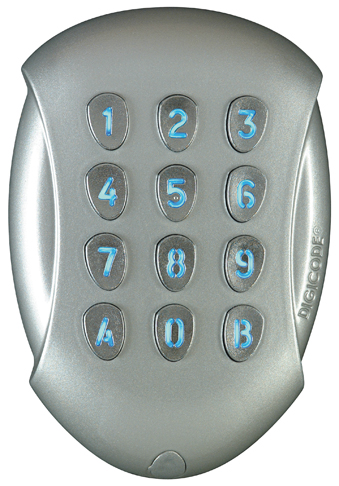
\includegraphics[width=.7\textwidth]{images/digicode}
%
%\textit{Digicode}
%\end{center}
%\end{minipage}\hfill
%\begin{minipage}[c]{.2\linewidth}
%\begin{center}
%%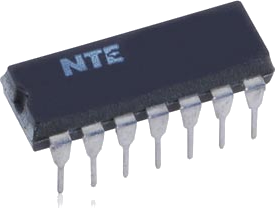
\includegraphics[width=.8\textwidth]{images/transistor_ttl_nand}
%
%\textit{Transistor TTL (permettant de réaliser des opérations logiques) }
%\end{center}
%\end{minipage}\hfill
%\begin{minipage}[c]{.2\linewidth}
%\begin{center}
%%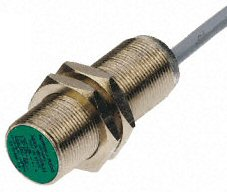
\includegraphics[width=.8\textwidth]{images/inductif}
%
%\textit{Détecteur inductif}
%\end{center}
%\end{minipage}\hfill
%\begin{minipage}[c]{.2\linewidth}
%\begin{center}
%%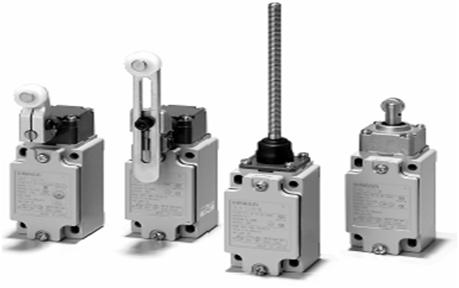
\includegraphics[width=\textwidth]{images/capteur_contact}
%
%\textit{Détecteur à contact}
%\end{center}
%\end{minipage}
%
%Un des objectifs de l'automaticien est de concevoir la partie commande qui traite les informations et élabore les ordres. Ce cours étudie le cas où les informations et les ordres élaborés sont des variables binaires.

Les systèmes à événements discrets sont des systèmes logiques. Ils diffèrent des systèmes combinatoires par la prise en compte d'une <<mémoire>> de l'état du système. En effet, alors que dans un système combinatoire, une même combinaison des entrées provoque les mêmes actions en sortie, dans les systèmes séquentiels, une même combinaison des entrées peut provoquer des sorties différentes (\textit{Exemple : interrupteur va-et-vient d'une installation électrique}).

\begin{savoir}
\textsc{Savoirs :}
\begin{itemize}
\item \textbf{Mod - C5.1 :} Modélisation des systèmes à événements discrets (fonctions logiques, tables de vérité).
\end{itemize}
\end{savoir}

%\newpage 

\setlength{\parskip}{0ex plus 0.2ex minus 0ex}
 \renewcommand{\contentsname}{}
 \renewcommand{\baselinestretch}{1}

\tableofcontents

 \renewcommand{\baselinestretch}{1.2}
\setlength{\parskip}{2ex plus 0.5ex minus 0.2ex}

% \vspace{1cm}
\textit{Ce document évolue. Merci de signaler toutes erreurs ou coquilles.}

\section{La fonction mémoire}

\subsection{Le chronogramme}
Le chronogramme est un outil permettant d'afficher l'état des entrées et des sorties en fonction du temps. Le chronogramme suivant indique le fonctionnement d'une lampe. L'interrupteur <<va-et-vient>> est relié à un relais. 

\begin{minipage}[c]{.47\linewidth}
\begin{center}
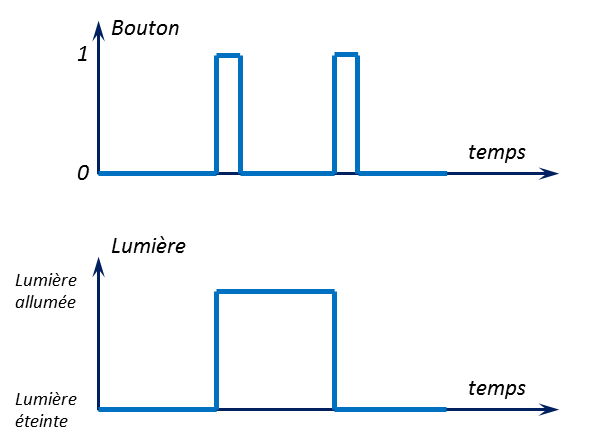
\includegraphics[width=.9\textwidth]{images/Chrono1}
\end{center}
\end{minipage} \hfill
\begin{minipage}[c]{.47\linewidth}
\begin{center}
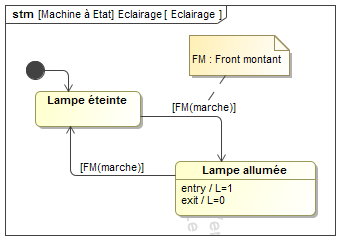
\includegraphics[width=.95\textwidth]{images/stm1}
\end{center}
\end{minipage}

Ainsi, pour une même combinaison des entrées, on observe des états différents de la sortie.

Le même constat peut être dresser à partir du fonctionnement d'un moteur (\textit{Exemple : fonctionnement du système Doshydro}).


\begin{minipage}[c]{.47\linewidth}
\begin{center}
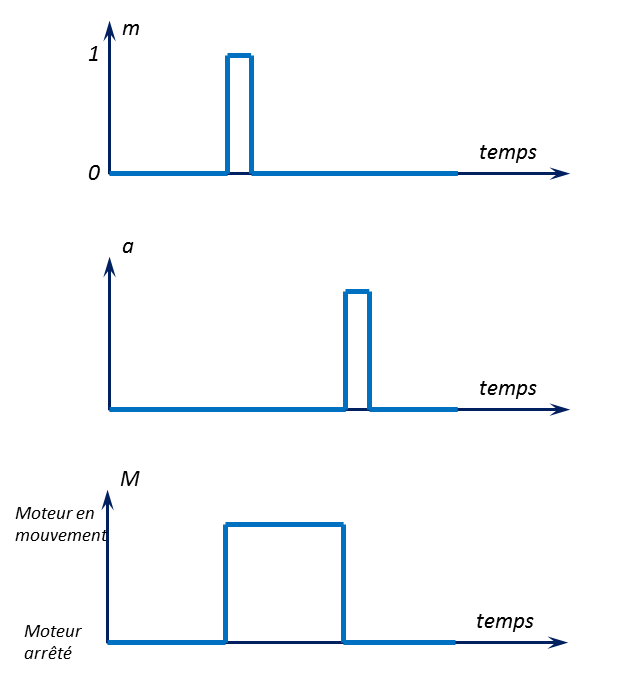
\includegraphics[width=.9\textwidth]{images/Chrono2}
\end{center}
\end{minipage} \hfill
\begin{minipage}[c]{.47\linewidth}
\begin{center}
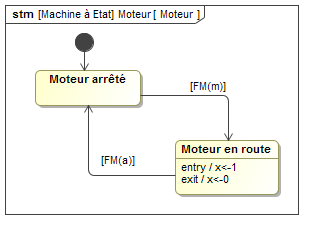
\includegraphics[width=.95\textwidth]{images/Moteur}

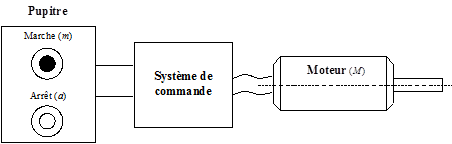
\includegraphics[width=.95\textwidth]{images/Moteur_im}
\end{center}
\end{minipage}

Ici aussi, on remarque qu'une même combinaison des entrées ($a=m=0$) peut conduire à un état de marche ou d'arrêt du moteur. Une variable interne, ici, une mémoire, permet de mémoriser l'état du moteur. 

\subsection{Notion de mémoire}

La mémorisation des états est à la base de l'existence des systèmes séquentiels. En notant $x$ la variable interne d'un système, on lui associe une mémoire.

 On peut noter l'existence des mémoires permanentes (qui conservent l'état des variables en cas de coupure d'énergie) et les mémoires volatiles (qui perdent l'état des variables en cas de coupure d'énergie).  
 
 Les mémoires peuvent être réalisées de façon optique (blue-ray), électropneumatiques (distributeurs électropneumatiques bistables), mangnétiques (disques durs), électriques (grâce à des transistors, mémoire flash), électromagnétique (relais). 
 
 Dans les systèmes automatisés industriels, le relais auto maintenu électromagnétique est un élément clef de la mémorisation des états. 

\begin{center}
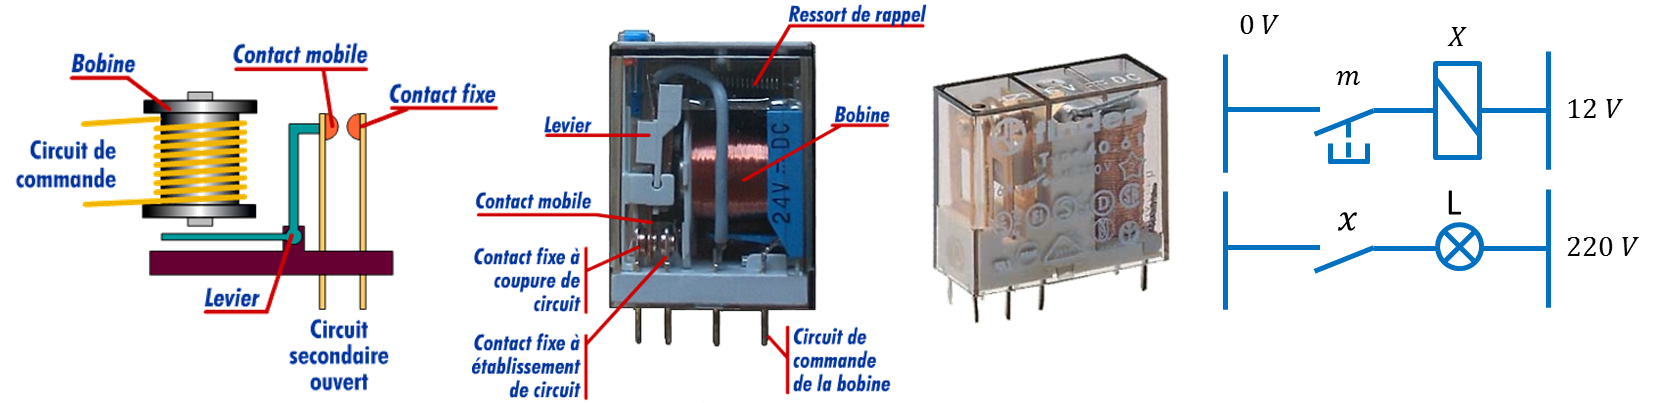
\includegraphics[width=\textwidth]{images/relais}
\end{center}

Lorsque l'utilisateur presse le bouton $m$, le relais $X$ est activé. Ainsi, la variable $x$ est mise à 1 ce qui provoque l'éclairage de la lampe $L$. \'A ce stade, si on relâche l'interrupteur $m$ le relais $X$ est désactivé, la variable $x$ passe à l'état 0 et la lampe s'éteint.

\begin{prob}
Comment réaliser une mémoire par l'utilisation d'un relais ? 

Que se passe-t-il lors de l'appui simultané sur marche et arrêt. 
\end{prob}

\subsection{Réalisation d'une mémoire}
\subsubsection{Mémoire à effacement prioritaire}
Dans ce cas, le moteur s'allume lorsque $m$ est pressé. Il est éteint lorsque $a$ est pressé ou lorsque $m$ et $a$ sont pressés simultanément.
 
 
\begin{minipage}[c]{.5\linewidth}
\begin{center}
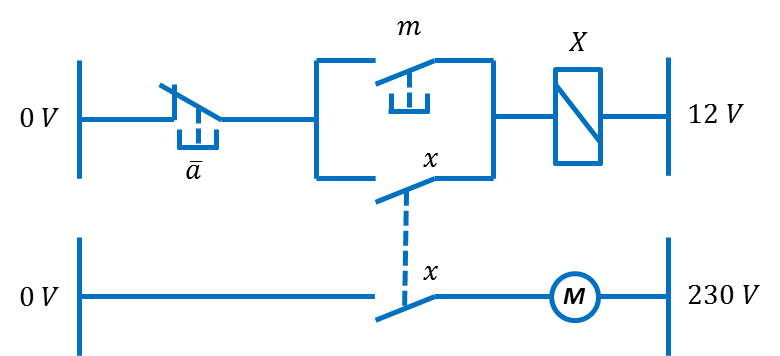
\includegraphics[width=\textwidth]{images/mem_eff}
\end{center}
\end{minipage} \hfill
\begin{minipage}[c]{.47\linewidth}
Il est possible de traduire le fonctionnement du moteur par l'équation booléenne suivante : 
$$
M = \overline{a} \cdot \left(m +  x \right)
$$
Ainsi dans un premier temps, en appuyant sur $m$ le relais est actionné, $x$ passe donc à 1 dans le circuit de puissance (allumant ainsi le moteur) \textbf{et} dans le circuit de commande. On effectue ainsi un \textbf{auto maintien}. 

On comprend aisément qu'un appui simultané sur $a$ et $m$ provoque une désactivation du relais et donc un arrêt du moteur. 
\end{minipage}

 Lorsqu'on utilise une technologie électronique, il est courant d'utiliser de réaliser un câblage en utilisant des cellules NOR. 

\vspace{.2cm}

\begin{minipage}[c]{.3\linewidth}
\begin{center}
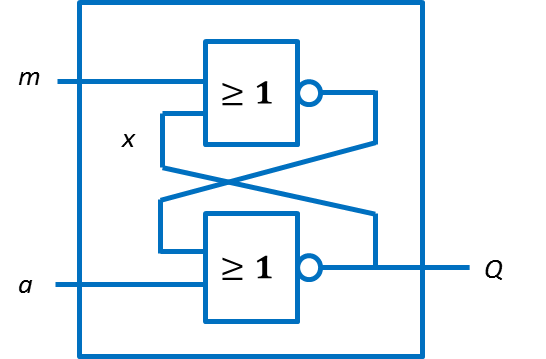
\includegraphics[width=\textwidth]{images/mem_eff_nor}
\end{center}
\end{minipage} \hfill
\begin{minipage}[c]{.2\linewidth}
\begin{center}
\begin{tabular}{|c|c|c||c|}
\hline
m & a & x & Q \\
\hline \hline
0 & 0 & 0 & 0 \\\hline
0 & 0 & 1 & 1 \\\hline
0 & 1 & 0 & 0 \\\hline
0 & 1 & 1 & 0 \\\hline
1 & 0 & 0 & 1 \\\hline
1 & 0 & 1 & 1 \\\hline
1 & 1 & 0 & 0 \\\hline
1 & 1 & 1 & 0 \\\hline
\end{tabular}
\end{center}
\end{minipage} \hfill
\begin{minipage}[c]{.48\linewidth}
Il  n'est pas directement possible d'écrire directement la table de vérité de la sortie $Q$ en fonction de $a$ et de $b$. Il faut avoir recours à une variable interne $x$. 

On retrouve bien l'équation précédente : 
$$
Q = \overline{m}\cdot \overline{a} \cdot x + \underbrace{m\cdot \overline{a} \cdot \overline{x} 
+ m\cdot \overline{a} \cdot x}_{m\cdot \overline{a} } = \overline{a} \left(\overline{m} \cdot x + m\right)
= \overline{a} \left( x + m\right)
$$

\end{minipage}

\paragraph*{Les bascules}
Le montage précédent est appelé une bascule SR (Set -- Reset). Suivant les cas d'utilisation, il en existe plusieurs. 
   
  
\vspace{.2cm}

\begin{minipage}[c]{.15\linewidth}
\begin{center}
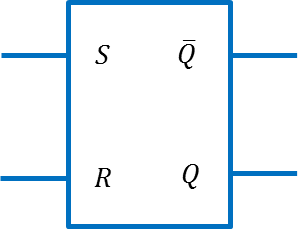
\includegraphics[width=\textwidth]{images/basculeRS}
\end{center}
\end{minipage} \hfill
\begin{minipage}[c]{.2\linewidth}
\begin{center}
\begin{tabular}{|c|c||c|c|}
\hline
$S$ & $R$ &  $Q_n$ & $\overline{Q_{n}}$ \\
\hline \hline
0 & 0 & $Q_{n-1}$ & $\overline{Q_{n-1}}$ \\ \hline
0 & 1 & 0 & 1 \\\hline
1 & 0 & 1 & 0 \\\hline
1 & 1 & 0 & 0 \\\hline
1 & 1 & -- & -- \\\hline
\end{tabular}
\end{center}
\end{minipage} \hfill
\begin{minipage}[c]{.53\linewidth}
La bascule RS est caractérisée par deux états : 
\begin{itemize}
\item S (Set) caractérise <<la mise à 1>>;
\item R (Reset) caractérise <<la mise à 0>>.
\end{itemize}

$Q_n$ et $\overline{Q_n}$ caractérisent les deux sorties stables. La combinaison $S=R=1$ est à éviter car elle conduit à des dysfonctionnement. Pour palier à ce problème, on utilise une bascule JK. 
\end{minipage}
   	
  \vspace{.2cm}
\hfill
\begin{minipage}[c]{.15\linewidth}
\begin{center}
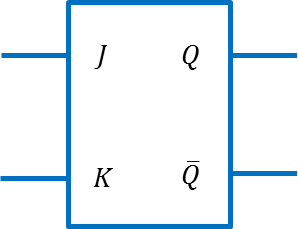
\includegraphics[width=\textwidth]{images/basculeJK}
\end{center}
\end{minipage} \hfill
\begin{minipage}[c]{.4\linewidth}
\begin{center}
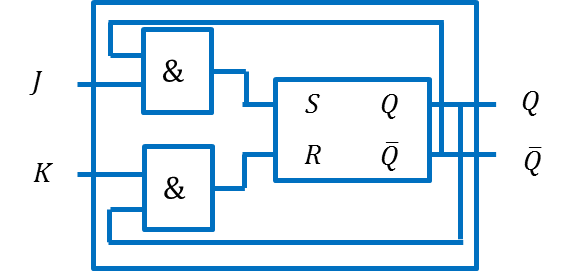
\includegraphics[width=\textwidth]{images/basculeJK_logi}
\end{center}

\end{minipage} \hfill
\begin{minipage}[c]{.35\linewidth}

\begin{center}
\begin{tabular}{|c|c||c|c|}
\hline
$J$ & $K$ &  $Q_n$ & $\overline{Q_{n}}$ \\
\hline \hline
0 & 0 & $Q_{n-1}$ & $\overline{Q_{n-1}}$ \\ \hline
0 & 1 & 0 & 1 \\\hline
1 & 0 & 1 & 0 \\\hline
1 & 1 & 0 & 0 \\\hline
1 & 1 & $Q_{n-1}$ & $\overline{Q_{n-1}}$ \\\hline
\end{tabular}
\end{center}
\end{minipage}\hfill

\section{Modélisation du comportement des systèmes séquentiels \cite{pb}}

Les outils privilégiés pour décrire le fonctionnement d'un système séquentiel seront les diagramme SysML. Le diagramme de séquence (CI 1 -- Chapitre 6) permet de présenter la succession d'étapes liés à un cas d'utilisation d'un point de vue utilisateur. Le diagramme d'état et le diagramme d'activité (CI 1 -- Chapitre 7 \& 8) permettent de décrire l'évolution interne du système. 
                           

\subsection{Construction et lecture d'un diagramme d'états}

\begin{methode}
  Pour chaque activité, il faut définir un état représenté par un noeud. Au cas où
aucune activité n’est souhaitée, c’est un état d’attente.

Il faut ensuite identifier les cas d’évolution du système, c'est-à-dire les transitions
possibles d’un état à un autre. On trace alors un lien entre les n\oe{}uds
correspondants. Chaque transition peut être qualifiée par un évènement, une
condition de garde et un effet.
\end{methode}

\begin{exemple}
\textit{Commande tout ou rien d'un moteur}

\begin{minipage}[c]{.48\linewidth}
Deux états internes du système cohabitent. Dans un cas le moteur est en marche, dans l’autre il est à l’arrêt.

Les conditions de passage d’un état à un autre se font à l’aide des variables d’entrée arrêt « a » et marche « m ».


L’activité « marche moteur » peut être détaillée dans un diagramme d’activité. Elle comporterait l’action « distribuer l’énergie ». Son exécution ne nécessite pas de temps significatif, elle est associée à un ordre de commande en direction du préactionneur du moteur (un contacteur électrique à arrêt prioritaire).
\end{minipage} \hfill
\begin{minipage}[c]{.48\linewidth}
\begin{center}
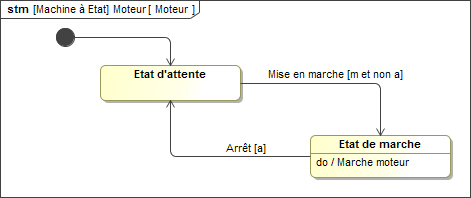
\includegraphics[width=\textwidth]{images/Moteur2}
\end{center}
\end{minipage}


\end{exemple}

\subsection{Utilisation des pseudo-états}


\begin{methode}
Les pseudo-états permettent d’utiliser des fonctionnalités avancées sans trop compliquer le diagramme d’état avec le formalisme de base.
Il est alors possible de montrer des sélections de séquences d’états (évolutions avec alternatives), des structures parallèles (évolutions simultanées), etc.
\end{methode}

\begin{exemple}

\textit{Commande tout ou rien (TOR) d’un moteur}

Un diagramme d’états « choix de mode » de niveau hiérarchique supérieur à celui décrit précédemment (« commande moteur »), permet de le démarrer selon deux modes :
\begin{itemize}
\item « mode normal » : moteur à l’arrêt dans l’« état d’attente »;
\item « mode historique » : dernier état avant que l’on sorte du diagramme « commande moteur » (« état d’attente » ou « état de marche »).
\end{itemize}

\begin{center}
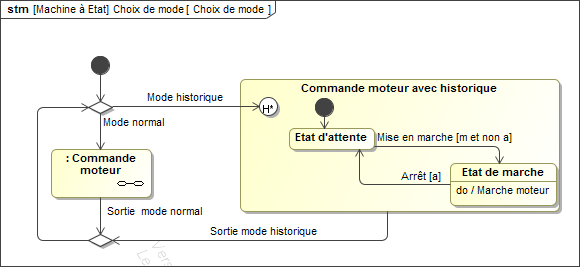
\includegraphics[width=.7\textwidth]{images/ChoixMode}
\end{center}
\end{exemple}

\section{Structures algorithmiques}
\subsection{Affectation}
L’affectation d’une valeur à une variable peut se faire à l’aide d’une action. Cela ne prend pas
de temps significatif.

\begin{minipage}[c]{.48\linewidth}
\begin{center}
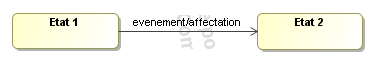
\includegraphics[width=\textwidth]{images/Affectation_stm}

\textit{Diagramme d'états -- Affectation}
\end{center}
\end{minipage} \hfill
\begin{minipage}[c]{.48\linewidth}
\begin{center}
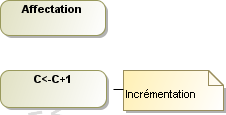
\includegraphics[width=.6\textwidth]{images/Affectation_act}

\textit{Diagramme d'activité -- Affectation}
\end{center}
\end{minipage}

\subsection{Groupe d'instructions}
\begin{minipage}[c]{.68\linewidth}
Un groupe ou un bloc d’instructions peut être une séquence d’un diagramme
d’activité. Cela correspond à une succession d’actions et / ou d’activités.
\end{minipage} \hfill
\begin{minipage}[c]{.3\linewidth}
\begin{center}
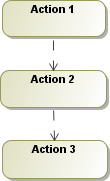
\includegraphics[width=.5\textwidth]{images/Groupe_act}

\textit{Diagramme d'activité -- Affectation}
\end{center}
\end{minipage}


\subsection{Fonctions et procédures}
La décomposition d’un algorithme en fonctions et procédures, permet :
\begin{itemize}
\item d’une part, de scinder une problématique générale en plusieurs problématiques
élémentaires;
\item d’autre part, de pouvoir réutiliser des sous-programmes réalisant des tâches élémentaires.
Une procédure comporte une succession d’instructions mais ne renvoie rien.
\end{itemize}


\begin{minipage}[c]{.48\linewidth}
\begin{center}
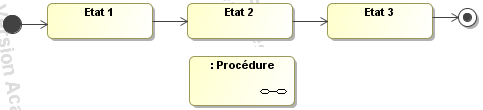
\includegraphics[width=\textwidth]{images/Fonctions_stm}

\textit{Diagramme d'états -- Affectation}
\end{center}
\end{minipage} \hfill
\begin{minipage}[c]{.48\linewidth}
\begin{center}
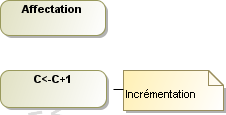
\includegraphics[width=.7\textwidth]{images/Affectation_act}

\textit{Diagramme d'activité -- Affectation}
\end{center}
\end{minipage}


A la fin de l’exécution d’une fonction, il y a le retour d’une valeur, d’une liste, d’un objet, etc.
\subsection{Structure alternative (conditionnelle)}

\begin{minipage}[c]{.48\linewidth}
\begin{center}
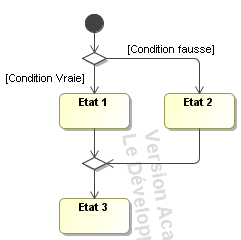
\includegraphics[width=.8\textwidth]{images/Condition_stm}

\textit{Diagramme d'états -- Structure alternative complète}
\end{center}
\end{minipage} \hfill
\begin{minipage}[c]{.48\linewidth}
\begin{center}
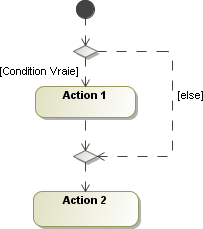
\includegraphics[width=.6\textwidth]{images/Condition_act}

\textit{Diagramme d'activité -- Structure alternative avec saut}
\end{center}
\end{minipage}

\subsection{Structure répétitive (itérative)}
\begin{minipage}[c]{.48\linewidth}
\begin{center}
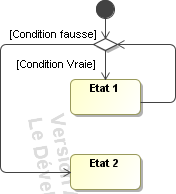
\includegraphics[width=.8\textwidth]{images/Iteratif_stm}

\textit{Diagramme d'états -- Tant que condition vraie faire ...}
\end{center}
\end{minipage} \hfill
\begin{minipage}[c]{.48\linewidth}
\begin{center}
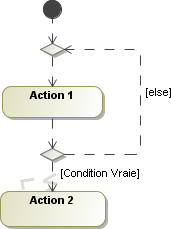
\includegraphics[width=.6\textwidth]{images/Iteratif_act}

\textit{Diagramme d'activité -- Répéter... jusqu'à condition vraie}
\end{center}
\end{minipage}


\begin{exemple}
Pour variable = valeur initiale, jusqu'à valeur maximale, faire...
\end{exemple}

\begin{minipage}[c]{.48\linewidth}
\begin{center}
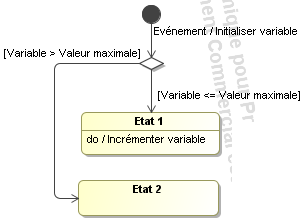
\includegraphics[width=.8\textwidth]{images/compteur_stm}

\textit{Diagramme d'états}
\end{center}
\end{minipage} \hfill
\begin{minipage}[c]{.48\linewidth}
\begin{center}
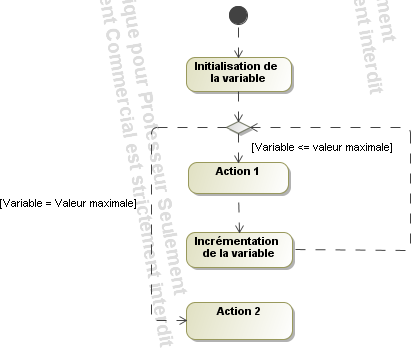
\includegraphics[width=.6\textwidth]{images/compteur_act}

\textit{Diagramme d'activité}
\end{center}
\end{minipage}

\begin{thebibliography}{2}
%\bibitem{dv}{Supports de cours de David Violeau, Lycée Saint-Louis, Paris.}
\bibitem{sg}{Stéphane Genouël, \textit{Systèmes Séquentiels -- Fonction mémoire}, Cours de MPSI -- PCSI, Lycée Chateaubriand, Rennes, \url{http://stephane.genouel.free.fr/}.} 
\bibitem{pb}{Patrick Beynet et Al., \textit{Sciences Industrielles pour l'Ingénieur, MPSI -- PCSI}, Éditions Ellipses.}
\bibitem{3}{Pierre Debout, \textit{Automatique -- Systèmes à événements discrets}, Cours de PCSI.}
\bibitem{4}{Thierry Schanen, \textit{Guide des automatismes 9.1}, Pos Industry, 2009.}
%\bibitem{fm}{Supports de cours de Florestan Mathurin, Lycée Bellevue, Toulouse.}
%\bibitem{jpp}{Supports de cours de Jean-Pierre Pupier, Lycée Rouvière, Toulon}

\end{thebibliography}

\end{document}\end{document}


